% \documentclass[pdflatex,11pt]{aghdpl}
% \documentclass{aghdpl}               % przy kompilacji programem latex
\documentclass[pdflatex,en]{aghdpl}  % praca w języku angielskim
\usepackage[british,UKenglish,USenglish,english]{babel}
\usepackage[utf8]{inputenc}

\usepackage[backend=bibtex,
%style=numeric,
bibencoding=ascii,
style=alphabetic
%style=reading
]{biblatex}

\addbibresource{bibliografia.bib}

% dodatkowe pakiety
\usepackage{enumerate}
\usepackage{listings}
\usepackage{float}
\usepackage{siunitx}

\lstloadlanguages{TeX}

\lstset{
  literate={ą}{{\k{a}}}1
           {ć}{{\'c}}1
           {ę}{{\k{e}}}1
           {ó}{{\'o}}1
           {ń}{{\'n}}1
           {ł}{{\l{}}}1
           {ś}{{\'s}}1
           {ź}{{\'z}}1
           {ż}{{\.z}}1
           {Ą}{{\k{A}}}1
           {Ć}{{\'C}}1
           {Ę}{{\k{E}}}1
           {Ó}{{\'O}}1
           {Ń}{{\'N}}1
           {Ł}{{\L{}}}1
           {Ś}{{\'S}}1
           {Ź}{{\'Z}}1
           {Ż}{{\.Z}}1
}

\newcommand{\rad}{\radian}

\usepackage{array}
\newcolumntype{L}[1]{>{\raggedright\let\newline\\\arraybackslash\hspace{0pt}}m{#1}}
\newcolumntype{C}[1]{>{\centering\let\newline\\\arraybackslash\hspace{0pt}}m{#1}}
\newcolumntype{R}[1]{>{\raggedleft\let\newline\\\arraybackslash\hspace{0pt}}m{#1}}

\makeatletter
\let\ps@plain\ps@fancy
\makeatother

%---------------------------------------------------------------------------

\author{Grzegorz Gajoch}
\shortauthor{G. Gajoch}

\titlePL{Budowa sensora pochłoniętej dawki promieniowania jonizującego (TID) dla nano-satelitów typu CubeSat}
\titleEN{Total Ionizing Dose (TID) sensor for CubeSat~nano-satellites}

\shorttitlePL{Budowa sensora pochłoniętej dawki promieniowania jonizującego (TID) dla nano-satelitów typu CubeSat} % skrócona wersja tytułu jeśli jest bardzo długi
\shorttitleEN{Total Ionizing Dose (TID) sensor for CubeSat~nano-satellites}

\thesistypePL{Praca inżynierksa}
\thesistypeEN{Bachelor of Science Thesis}

\supervisorPL{dr inż. Cerazy Worek}
\supervisorEN{Cerazy Worek Ph.D}

\date{2016}

\departmentPL{Katedra Elektroniki}
\departmentEN{Department of Electronics}

\facultyPL{Wydział Informatyki, Elektroniki i Telekomunikacji}
\facultyEN{Faculty of Computer Science, Electronics and Telecommunications}

\acknowledgements{Serdecznie dziękuję \dots tu ciąg dalszych podziękowań np. dla promotora, żony, sąsiada itp.}


%---------------------------------------------------------------------------

\begin{document}

\titlepages

\tableofcontents
\clearpage


\include{01_introduction}
% Introduction

\chapter{Terms, definitions and abbreviated terms}

\section{Abbreviated terms}

\section{Conventions}

% Terms, definitions and abbreviated terms
% - Abbreviated terms
% - Conventions

\chapter{Principles}

\section{Radiation effects on electronic devices}
    There are two basic effects of radiation on silicon components:
    \begin{itemize}
        \item ionizing effect
        \item displacement damage
    \end{itemize}

    Those two effect are responsible for changing parameters of semiconductor devices, which after some time can lead to failure of the device. Main source of this radiation are Gamma (ionization) and Neutron particles (displacement).

    In space electronics during analysis and design two major problems are considered - Single Event Effects (SEE) and Total Ionizing Dose (TID). Every silicon and silica device is susceptible to both of those - and both have to be considered during product design, development and testing.

    \subsection{Single Events Effects}
        Single Event Effects are connected with generation of electron-hole pair in semiconductor, when material is exposed to ionizing radiation. Amount of pairs generated is proportional to energy deposited. For semiconductor device parameter $LET_{th}$ (Linear Energy Transfer Threshold) is defined, being a measure of how susceptible the device is. For particles with Linear Energy Transfer (LET - normalized particle energy per mass of the absorbing material), below this threshold no effect will be observed.

        Single Event Effects are divided into two groups - non-destructive (fully recoverable, possibly after power cycle) and destructive (permanent damage) effects. Shortly those are described below, defined as in \cite{ECSS_Q_ST_60_15C}.

        \bigskip\textbf{Non-destructive effects}
        \begin{itemize}
            \item \textbf{Single Event Upset} - especially memory-based devices (like microprocessors, memories, Field Programmable Gate Array - FPGA) are vulnerable. This phenomenon will possibly alter the state of cell in memory - causing memory corruption. This can lead to complete failure of device if this is not corrected.

            \item \textbf{Single Event Functional Interrupt} - subset of SEU - this effect cause the system to latch in non-recoverable state (e.g. by switching to wrong state in state machine). Only option is to reset circuit to back to known state.

            \item \textbf{Single Event Transient} - are formed as a voltage/current spurious pulses generated by charge induced by striking particle. This can cause different problems - from disturbing analog electronics up to causing switch of digital circuit. This effect strongly depends on size of feature in silica.
        \end{itemize}

        \bigskip\textbf{Destructive effects}
        \begin{itemize}
            \item \textbf{Single Event Latch-up} - particle striking can cause turning on parasitic thyristor in CMOS structure. This will lead to effectively shorting voltage supply to ground, causing overheat and damage to the device.

            \item \textbf{Single Event Gate Rupture} - high energy particle comes through thin gate (especially in MOS transistors) can cause generation of electron-holes pairs in gate and substrate - causing high electric field across gate. When this effect is strong enough it can cause permanent damage to transistor.

            \item \textbf{Single Event Burnout} - ion that traverses the transistor structure (through the source) can induce a current flow that turns on the parasitic npn transistor. This leads to effective short circuit and damage to the device.
        \end{itemize}

        \bigskip\textbf{Mitigation techniques}

        Below recommended mitigation techniques for SEE were listed:
        \begin{itemize}
            \item SEU - redundancy, memory scrubbing,
            \item SEFI - watchdog, proper reset sequence,
            \item SET - use lower-integration scale devices, implement protection resistors etc.
            \item SEL - implement overcurrent circuits (like Latch-up Current Limiters),
            \item SEGR, SEB - use higher $LET_{th}$ devices
        \end{itemize}

    \subsection{Total Ionizing Dose}
        TID is defined as total energy absorbed during exposure. This can be caused by any kind of radiation, behaving differently in every semiconductor device. In general, TID successively degrades electronic device parameters in time, causing them to stop functioning when critical irradiation was reached. Effect in p-MOSFET transistor is described in section \ref{Radiation_effects_on_MOS_transistors}.

        Every qualified device for spacecraft system will have tested value of TID value, for example by MIL-STD-883G, Test Method 1019.7 \cite{MIL_STD_883}. For example, ADC128S102QML-SP have a guaranteed value of 100 kRad.

\section{Need for TID radiation dosimetry}
    During spacecraft mission accumulated radiation level should be monitored to not excess guaranteed values for components. For example, near end of its lifetime, spacecraft can be commanded to deorbit into atmosphere or move to parking orbit - before fail can occur, causing losing control of spacecraft.
    Absorbed dose simulation and estimation is possible, but results are averaged by long period of time. Constantly flying by South Atlantic Anomaly or Van Allen belts can cause radiation estimation to be inaccurate, so near all spacecrafts implement sensor which constantly monitor radiation level absorbed by its electronics.

\section{On-line TID radiation dosimetry}

\section{RadFET Theory}

    \subsection{Radiation effects on MOS transistors}
    \label{Radiation_effects_on_MOS_transistors}

    \subsection{Threshold voltage measurement}

    \subsection{Temperature dependencies}

% Principles
% - Ionising radiation
% - Radiation effects on electronics
% -- Single Events Effects
% -- Total Ionising Dose
% - Need for TID radiation dosimetry
% - On-line TID radiation dosimetry
% - RadFET Theory
% -- Radiation effects on MOS transistors
% -- Threshold voltage measurement
% -- Temperature dependencies

\chapter{Design requirements}
\label{Design_requirements}

In this chapter the requirements for the TID sensor will be presented.

The finalised sensor is to be flown on-board the PW-Sat2 CubeSat satellite. Therefore, it should be designed for these particular requirements. In addition, it should be designed with active space standard and launcher requirements in mind. Additional requirements come from CubeSat Design Specification, which summarizes them for CubeSat type satellite \cite{CDS}.

\section{PW-Sat2}
    The presented sensor is scheduled to be launched on the PW-Sat2 satellite \cite{PW-Sat2URL}. Therefore it should be designed especially for this particular type of mission. In this section the PW-Sat2 mission will be presented.

    PW-Sat2 is scheduled to be launched on Falon9 rocket from SpaceX company in Q4 2017.

    \begin{figure}[H]
        \centering
        \includegraphics[width=0.3\paperwidth]{img/04/Falcon9.jpg}
        \caption{Falcon9 rocket. Source: \cite{Falcon9_img}}
        \label{Falcon9}
    \end{figure}

    In the figure \ref{PW-Sat_render_01} an exploded render of PW-Sat2 is presented.

    \begin{figure}[H]
        \centering
        \includegraphics[width=0.65\paperwidth]{img/04/PW-Sat2_render_01.png}
        \caption{PW-Sat2 render. Source: \cite{PW_sat2_photo}}
        \label{PW-Sat_render_01}
    \end{figure}




    \subsection{Primary mission}
        The primary mission of PW-Sat2 is to test the deorbit sail. When satellite mission ends, it has to be safely deorbited (or moved to graveyard orbit). Due to new regulations, satellite has to be removed from
        the LEO region no later than 25 years after the end of vehicle operations \cite{Satellite_disposal}. Purpose of deorbit sail is, after satellite operations, to open and increase atmospheric drag, shortening satellite life and cause deorbitation. More information about this experiment can be found in \cite{DDC_article}.

        A render of PW-Sat2 with opened sail is shown in the figure \ref{PW-Sat_render_sail}.

        \begin{figure}[H]
            \centering
            \includegraphics[width=0.38\paperwidth]{img/04/PW-Sat2_render_02.png}
            \caption{PW-Sat2 with opened sail. Source: \cite{PW_sat2_photo}}
            \label{PW-Sat_render_sail}
        \end{figure}

    \subsection{Lifetime}
        Due to its primary mission, the basic lifetime of PW-Sat2 is planned to be 40 days long. After this time the deorbit sail will be opened and orbit will slowly decay. Deorbitation from nominal orbit is planned to take about one year \cite{PWSAT_MA_CDR}, but possibly with an unreliable data connection. Therefore the sensor should be able to measure the dose absorbed during the primary mission (40 days), but also to work throughout the full predicted mission - about one year.

    \subsection{Orbit}
        PW-Sat2 in planned to be launched to a sun-synchronous circular orbit of attitude \SI{575}{\kilo\meter}, with LTAN of 10:30 \cite{PWSAT_MA_CDR}.


    \subsection{Radiation analysis}
        Simulations in SPENVIS \cite{SPENVIS_URL} were performed to estimate TID accumulated during the PW-Sat2 mission. In the figure \ref{TIDvsSheilding} dose as a function of shielding thickness was plotted, during year-long mission on predicted orbit.

        \begin{figure}[H]
            \centering
            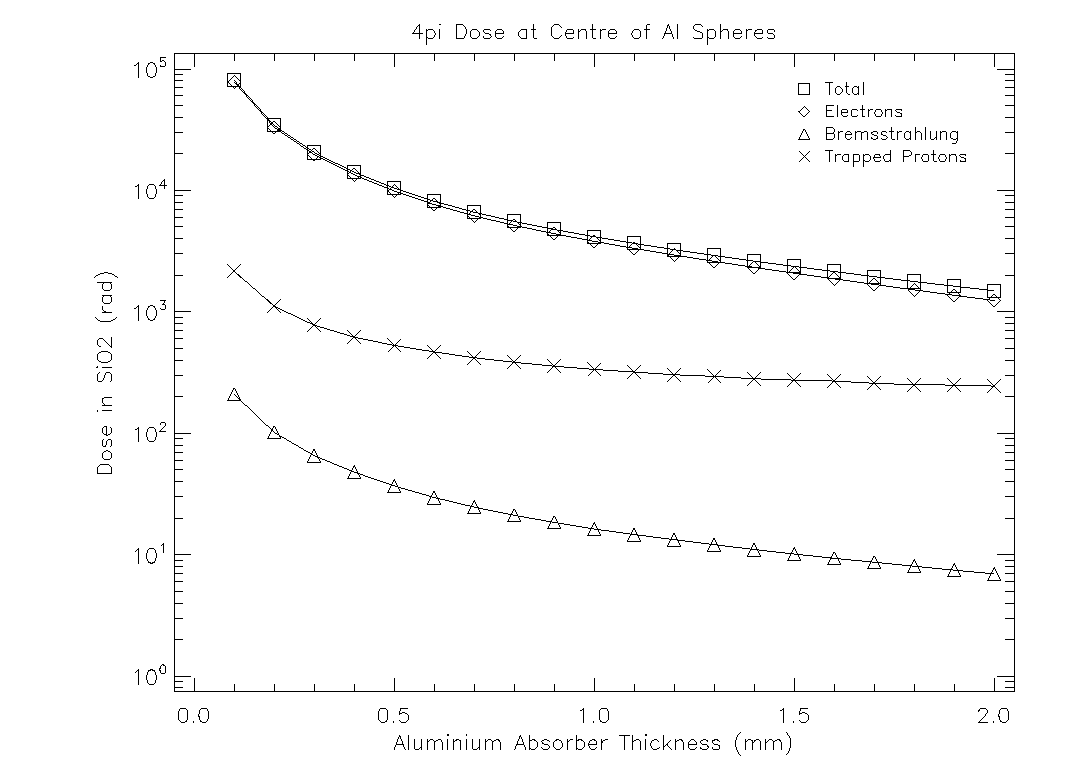
\includegraphics[width=0.58\paperwidth]{img/04/dose.eps}
            \caption{TID vs shielding during one year mission on \SI{575}{\kilo\meter} orbit}
            \label{TIDvsSheilding}
        \end{figure}

        The shielding of PW-Sat2 is about \SI{0.5}{\milli\meter} thick (aluminum sides as well as aluminum substrate for solar cells - \ref{PW-Sat_render_01}). Therefore, predicted dose during the primary mission is \SI{1}{\kilo\rad} and over the full, one year mission, is about \SI{10}{\kilo\rad}.

\section{Sensor requirements}
    Summing PW-Sat2 mission analysis, high-level sensor requirements were estimated, summarized in the table \ref{sensor_requirements_table}.

    \begin{table}[H]
        \caption{Sensor requirements}
        \label{sensor_requirements_table}
        \begin{center}
            \begin{tabular}{r|l}
                \textbf{Requirement} & \textbf{Value} \\ \hline
                Range & \SI{10}{\kilo\rad} \\
                Resolution & \SI{10}{\rad} \\
                Total accuracy & \SI{\pm 100}{\rad}
            \end{tabular}
        \end{center}
    \end{table}

\section{Applicable standards}
    The sensor should comply to ECSS \cite{ECSS_URL} standards. They are required by the launch provider and describe good practice during space product development.

    ESCIES \cite{ESCIES_URL} provides valuable knowledge about component qualification, testing and verification.

\section{Electrical requirements}
    The sensor will be placed on-board PW-Sat2. Therefore it should comply to its standards - power supplies, communication interfaces etc.

    \subsection{Electronics stack}
        Modules on PW-Sat2 are connected in the PC-104 stack structure as shown in the figure \ref{PW-Sat2_stack}. Is is placed inside the satellite housing and consists of (from the top):
        \begin{itemize}
            \item \textbf{Payload module (PLD)} - where the sensor will be located,
            \item On-Board Computer (OBC) - main data processing unit,
            \item Attitude Determination and Control Subsystem (ADCS) - controls attitude (detumbling and sunpointing),
            \item Electrical Power System (EPS) - charges and discharges batteries, provides safety mechanisms,
            \item Battery module (ACC) - main energy storage,
            \item Communication transceiver (COMM) - VHF \& UHF full duplex transceiver,
            \item Antennae module (ANT) - antennae for uplink and downlink.
        \end{itemize}

        \begin{figure}[H]
            \centering
            \includegraphics[width=0.5\paperwidth]{img/04/PW-Sat2-stack.png}
            \caption{PW-Sat2 electronics stack}
            \label{PW-Sat2_stack}
        \end{figure}

    \subsection{PC-104 connector}
        PLD board is connected to OBC with PC-104 connector. This connector provides data and power connections to the satellite bus.

        The connector consists of:
        \begin{itemize}
            \item $I^2C$ bus, connected directly to MCU on OBC,
            \item interrupt line on which the sensor can notify OBC about command completion,
            \item SENS \SI{5}{\volt} line, powered only when sensor is commanded to be enabled.
        \end{itemize}

    \subsection{Power rail}
        As mentioned earlier, the power for the sensor is +\SI{5}{\volt}, activated whenever the sensor is to be accessed by OBC.

        The power line is controlled and protected by a Latchup-Current Limiter FPF2701MX placed on the EPS board. Therefore, additional latchup protection in not necessary in this design. However, this sensor will not be the only one on the PLD board and should have its own power switch. The PLD board is enabled and disabled by EPS on the OBC command and the sensor should be enabled only during TID readout. Having this in mind forces the design to be immune to immediate shutdowns and dose have to be accumulated off-line.

    \subsection{Power consumption}
        During irradiation sensor should be completely turned off. It decreases possibility of radiation damage and increases overall system reliability.

        During readout the required power should be less than \SI{1}{W}.

    \subsection{Data interface}
        The sensor is connected to the OBC via the $I^2C$ interface. On this bus, OBC is the master, while the sensor is one of the slaves. The PLD board can be disabled and can therefore provide isolation of the $I^2C$ bus when it is powered off.

    \subsection{Radiation immunity}
        The design should itself be immune to radiation. For PW-Sat2, a threshold of \SI{10}{\kilo\rad} was chosen for all COTS components. Semiconductors should have radiation tests as described in \cite{ESCIES_TID_test_method}.

    \subsection{Electromagnetic compatibility}
        EMC requirements are described in \cite{ECSS_E_ST_20_07C}. This standard was tailored to PW-Sat2 because the power rail is \SI{+5}{\volt}, rather than the (\SI{+28}{\volt}) featured on bigger spacecraft.

        \begin{itemize}
            \item Conducted susceptibility is shown in the figure \ref{EMC_conducted_susceptibility} . It was created by down-scaling figure A-4 from \cite{ECSS_E_ST_20_07C} by factor of $\SI{28}{\volt}/\SI{5}{\volt} = 5.6$. The EMC limit on the power line is defined as a constant \SI{175}{\milli\volt} from \SI{30}{\hertz} to \SI{100}{\kilo\hertz}. The sensor should be able to filter this ripple to produce stable power for analog devices. In addition, it should be taken into account that output DC-DC converters on EPS run at \SI{500}{\kilo\hertz}.

            \begin{figure}[H]
                \centering
                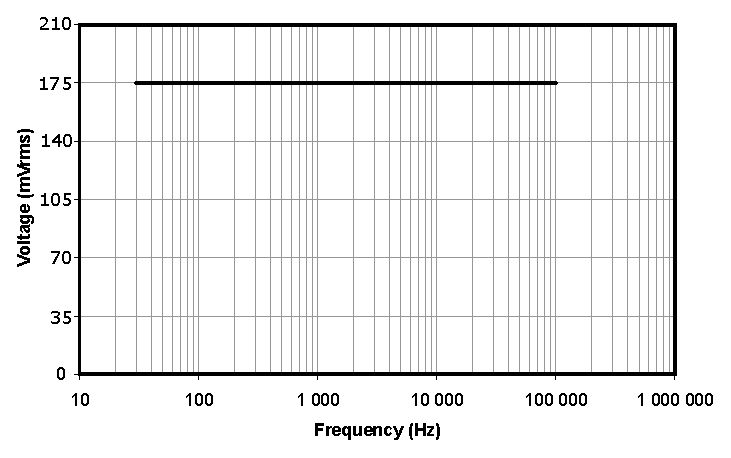
\includegraphics[width=0.5\paperwidth]{img/04/EMC_conducted_susceptibility.eps}
                \caption{Conducted susceptibility limit, frequency domain. Source: \cite{ECSS_E_ST_20_07C}}
                \label{EMC_conducted_susceptibility}
            \end{figure}


            \item Conducted emission is defined in the figure \ref{EMC_conducted_emission}.

            \begin{figure}[H]
                \centering
                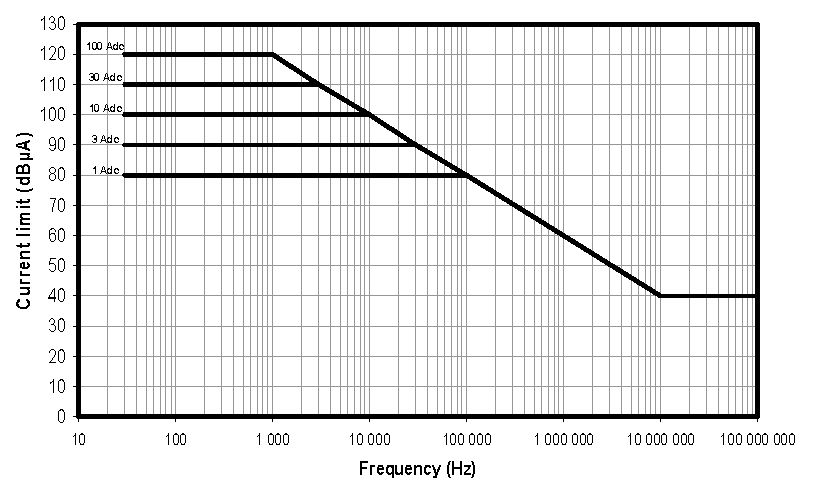
\includegraphics[width=0.5\paperwidth]{img/04/EMC_conducted_emission.eps}
                \caption{Conducted susceptibility limit, frequency domain. Source: \cite{ECSS_E_ST_20_07C}}
                \label{EMC_conducted_emission}
            \end{figure}


            \item Radiated susceptibility.
                On board PW-Sat2 is a communication module transmitting \SI{0.5}{\watt} of power at \SI{435.02}{\mega\hertz}. It is planned that during readout, the radio transmitter will be disabled, but proper tests should be conducted to check for possible errors and faults.

                PLD board is placed near OBC - so radiated emissions from digital lines can potentially couple to sensor elements causing noise and errors. Proper tests will be conducted and if necessary shielding will be implemented.

            \item Radiated emission.
                The sensor is not predicted to emit any kind of radio waves. In case of any detected anomalies, further design decisions would have to be made.

        \end{itemize}


    \subsection{Inrush current}
        Inrush current has to be limited to maximum power consumption to not trigger LCL on EPS (\SI{0.5}{\ampere}).

    \subsection{Reliability of components}
        This sensor is not a critical part of the satellite. Nonetheless, reliable components should be used to ensure proper results.

        Every used component should have a failure rate of $0.1\si{\percent}$ or lower. This is essential in capacitors and other passive components.

\section{Mechanical requirements}
    In this chapter design constraints and mechanical requirements of Falcon9 are presented. Launcher requirements were taken from \cite{Falcon9_user_manual}.

    \subsection{PCB}
    \label{PCB_description}
        PCB of PLD board is standard 4-layer FR4 board with stack shown in the figure \ref{PLD_PCB_stack}. Its dimensions are shown in the figure \ref{PLD_PCB_size}. The sensor design must, of course, occupy only a small amount of space on the board. For the sensor footprint, the limits are \SI{3x3}{\centi\meter} double sided.

        \begin{figure}[H]
            \centering
            \includegraphics[width=0.7\paperwidth]{img/04/PLD_PCB_stack.png}
            \caption{PLD board PCB stack}
            \label{PLD_PCB_stack}
        \end{figure}

        \begin{figure}[H]
            \centering
            \includegraphics[width=0.7\paperwidth]{img/04/PC104_PLD_size.png}
            \caption{PC-104 size}
            \label{PLD_PCB_size}
        \end{figure}



    \subsection{Outgassing}
        Every component used should be able to work in vacuum. Outgassing of components should be known to conduct required vacuum tests before launch. Too great an outgassing coefficient can result in damage to the turbomolecular pump in the vacuum chamber.

    \subsection{Vibration}
        During the rocket launch, large vibrations occur on the payload, therefore the rocket payload should be immune to vibration. In the case of heavy electronic components, appropriate glue should be applied to prevent joint cracks.
        \begin{figure}[H]
            \centering
            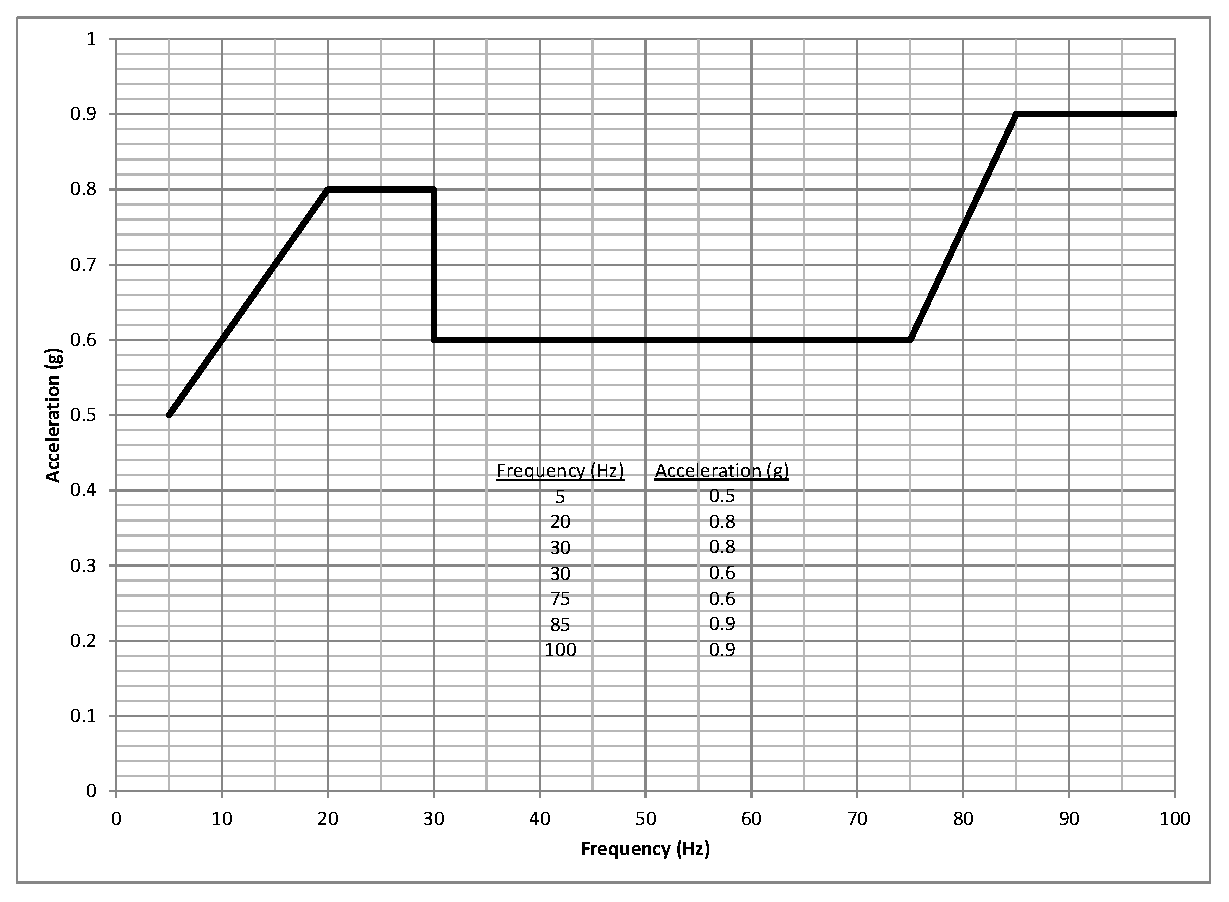
\includegraphics[width=0.5\paperwidth]{img/04/Falcon9_vibration.eps}
            \caption{Falcon9 maximum axial equivalent sine environment. Source: \cite{Falcon9_user_manual}}
            \label{Falcon9_vibration}
        \end{figure}


    \subsection{Operation temperature}
        The sensor should work in every operational case a satellite can be. Simulations were performed to find the boundaries of the  possible temperature range inside the satellite.    In \cite{PWSAT_TCS_CDR} results are presented.

        For the PLD board, the operation range is $\SI{0}{\degreeCelsius}$ to $\SI{60}{\degreeCelsius}$. If the measured temperature is outside this range, the sensor will not be enabled.


    \subsection{Thermal cycles}
        On the PW-Sat2 orbit, the sun illumination is changing every $\approx \SI{90}{\minute}$. Therefore a large number of thermal cycles are applied to the On-Board electronics, which can cause joint cracks as well as component failures. Proper soldering and component selection will be made, according to ECSS.

        As described in \cite{ECSS_Q_ST_70_04C} the sensor should pass thermal cycle tests: $100$ times from $- (100 \pm 5)$\si{\degreeCelsius} to $(100 \pm 5)$\si{\degreeCelsius} in a vacuum environment. This will be tested on Qualification Model.

% Design requirements
% - Sensor requirements
% -- Required sensitivity
% -- Required accuracy
% - Applicable standards
% - PW-Sat Mission
% -- Main purpose
% -- Orbit \& lifetime
% -- Radiation analysis
% - Electrical requirements
% -- Electronics stack
% -- Power
% -- Data interface
% -- Radiation immunity
% -- Reliability of components
% - Mechanical requirements
% -- PCB stack \& PCB restrictions
% -- Space available
% -- Vibration
% -- Operation temperature
% -- Thermal cycles

\chapter{Sensor design}
This chapter will cover sensor element selection, according to requirements presented previously.

Most space missions have on-board TID sensor - based od RadFET. RadFET is special type of modified p-MOSFET transistor, with well known dose dependence. In research work many COTS elements were checked for their characteristics, and they are now considered as a RadFET equivalent.

\section{RadFETs}
    Commercial solutions are based on modified MOS structure (with thicker gate region). Example silicon structure is show in figure \ref{Tyndall_radfet_silicon}. Different companies produce their own RadFET devices, by designing different structure, fitted to particular requirements. Found companies produce RadFET sensor alone, leaving readout circuit design for customer. Physical phenomena for RadFET sensors is described in section \ref{Physical_phenomena_background}.

    \begin{figure}[H]
        \centering
        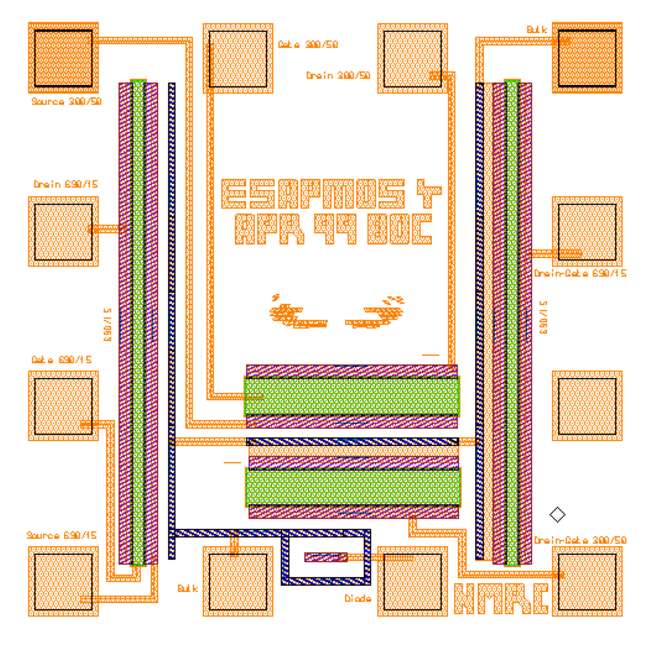
\includegraphics[width=0.5\paperwidth]{img/radfet-silicon.eps}
        \caption{4x RadFET silicon structure by Tyndall. Source: \cite{Tyndall_Radfet}}
        \label{Tyndall_radfet_silicon}
    \end{figure}


    Available products on market:

    \subsection{REM Oxford}
        REM Oxford \cite{RADFET_COM_URL}. This company produces RadFET type RFT300-CC10G1, its datasheet can be found on \cite{RFT300_CC10G1}. Structure is mounted on small carrier, as shown on figure \ref{REM_radfet_drawing}.

        \begin{figure}[H]
            \centering
            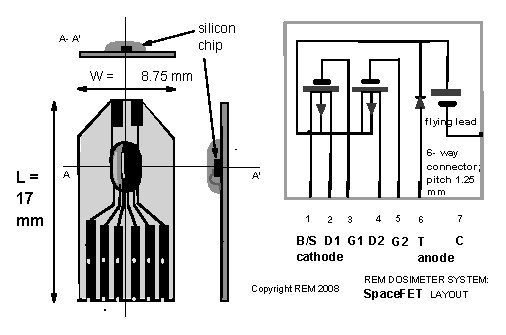
\includegraphics[width=0.5\paperwidth]{img/remOxfordDrawing.eps}
            \caption{RadFET made by REM Oxford. Source: \cite{RFT300_CC10G1}}
            \label{REM_radfet_drawing}
        \end{figure}

        This sensor consists of two PMOS transistors with modified gate structure.

        Key features:
        \begin{itemize}
            \item gate thickness \SI{200}{\nano\meter}, \SI{250}{\nano\meter} or \SI{300}{\nano\meter},
            \item sensitivity $\SI{1.5}{\milli\volt/\centi\gray} = \SI{1.5}{\milli\volt/\rad}$. Sensitivity chart is shown on figure \ref{REM_radfet_sensitivity}. At required sensitivity (\SI{1}{kRad}) threshold voltage shifts by $>\SI{100}{\milli\volt}$, depending on configuration,
            \item fading of shift is shown on figure \ref{REM_radfet_fading} - it is negligible on required mission duration ($<~\SI{3}{\percent}$),
            \item manufacturer suggests readout current in range $10-\SI{500}{\micro\ampere}$,
            \item sensor includes temperature readout from on-die diode
        \end{itemize}

        Price for one RadFET sensor begins from 800~\$.

        \begin{figure}[H]
            \centering
            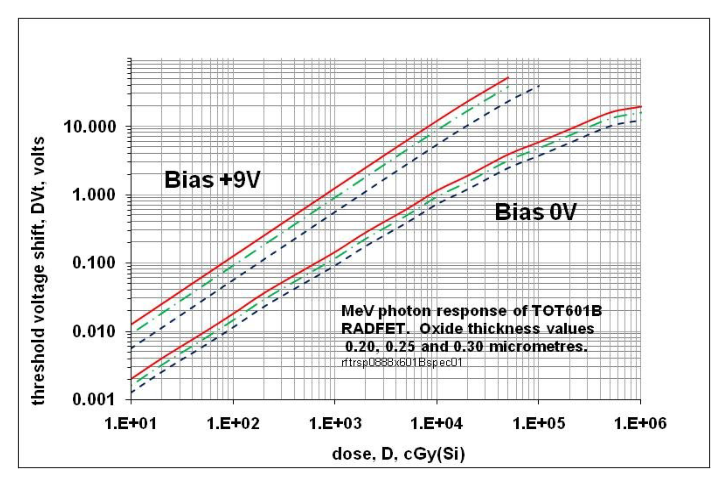
\includegraphics[width=0.6\paperwidth]{img/remSensitivity.eps}
            \caption{REM Oxford RadFET sensitivity. Source: \cite{RFT300_CC10G1}}
            \label{REM_radfet_sensitivity}
        \end{figure}

        \begin{figure}[H]
            \centering
            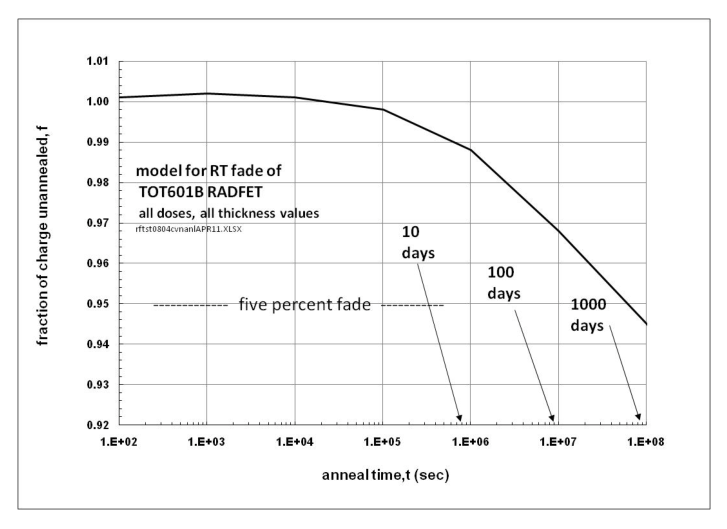
\includegraphics[width=0.6\paperwidth]{img/remOxfordFading.eps}
            \caption{REM Oxford RadFET fading. Source: \cite{RFT300_CC10G1}}
            \label{REM_radfet_fading}
        \end{figure}


    \subsection{Tyndall}
        Tyndall Works manufactures RadFET components in different packaging options \cite{TYNDALL_URL}. They provide calibration data for each type of sensor, as their response is very non-linear. Graph showing sensitivity of TY1002 is shown on figure \ref{Tyndall_TY1002_sensitivity}. Tyndall provide 4 different options, their comparison is done in table \ref{Tyndall_comparison}. Tyndall recommends grounding RadFET terminals during irradiation.

        \begin{figure}[H]
            \centering
            \includegraphics[width=0.6\paperwidth]{img/Tyndall_TY1002_sensitivity.png}
            \caption{Tyndall TY1002 sensitivity. Source: \cite{TYNDALL_URL}}
            \label{Tyndall_TY1002_sensitivity}
        \end{figure}

        \begin{table}[H]
        \begin{tabular}{| L{3.5cm} | C{2.5cm} | C{2.5cm} | C{2.5cm} | C{2.5cm} |}
            \hline
            Type: & TY1001 & TY1002 & TY1003 & TY1004 \\ \hline

            Image: &
            \includegraphics[width=0.12\paperwidth]{img/TY1001.png} &
            \includegraphics[width=0.12\paperwidth]{img/TY1002.png} &
            \includegraphics[width=0.12\paperwidth]{img/TY1003.png} &
            \includegraphics[width=0.12\paperwidth]{img/TY1004.png} \\ \hline

            Package: & 14-pin ceramic DILpin ceramic DIpin ceramic DI & SOT-23 & SOT23-6 & 8-pin ceramic DIL \\ \hline

            \# of transistors: & 4 & 1 & 2 & 2 \\  \hline
            W/L : & 300/50 \& 690/15 & \multicolumn{3}{c|}{300/50}  \\  \hline
            Oxide thickness: & - & - & \multicolumn{2}{c|}{\SI{400}{\nano\meter}} \\  \hline

            Maximum dose: & \multicolumn{4}{c|}{\SI{100}{\kilo\rad}} \\  \hline
            Minimal detectable dose: & \multicolumn{4}{c|}{\SI{1}{\rad}} \\  \hline

            Recommended readout current: & \multicolumn{2}{c|}{\SI{12.5}{\micro\ampere}} & \multicolumn{2}{c|}{\SI{10}{\micro\ampere}} \\ \hline

            Temperature readout: & diode & none & diode & diode \\ \hline
        \end{tabular}
        \caption{Tyndall RadFET comparison}
        \label{Tyndall_comparison}
        \end{table}


\section{MOSFET as RadFET}
    COTS transistors parameters also depends on total dose - but in less predictable way. But this solution is much cheaper, and after self-made calibration can be considered as flight solution. According to papers, many transistors were already measured by different scientific teams. For this thesis couple of them were selected for comparison.

    P-MOSFET can have different characteristics (lower slope, higher drift and fading) than commercial RadFETs, but considering cost and space it is unfeasible for implementing RadFET-based sensor on PW-Sat2.



\section{Chosen MOSFET: CD4007}

\section{Conceptual Block diagram}

    Conceptual block diagram is presented on figure TODO. It consists of mosfet, current source, analog to digital converter and die temperature measurement. Description is presented below.

    \subsection{Thresold voltage}
        According to theory, to measure TID accumulated threshold voltage in transistor have to be measured. The simplest solution is to use current source connected to MOSFET in diode connection. Measured voltage is not true threshold voltage which literature refers to, but this is enough for TID measurements, because absolute value of $V_{th}$ does not matter - only it's shift. From now, this thesis will refer to $V_{th}$ defined as $V_{GS}$ at a given drain current.

        During irradiation current source should be disabled - as well as the whole sensor. This will lead to no power consumption during irradiation, enabling device only for readout.

    \subsection{Die temperature}
        Because measured threshold voltage strongly depends on die temperature this effect have to be compensated. According to papers, predicted dependence $V_{th}(TID)$ is about $TODO$ and temperature shift is \SI{-2}{\milli\volt/\kelvin}. Therefore die temperature have to be measured very accurately, and individual MOSFET will have to be calibrated prior to launch.

        Couple of options were considered during this thesis:
        \begin{itemize}
            \item discrete PT-1000 sensor glued to MOSFET - this was rejected because of large heat resistance,
            \item ESD diode measurement in CD4007 - readout circuit for this solution is rather complicated, therefore it was rejected too,
            \item body diode in N-MOSFET in CD4007 package - this is chosen solution
        \end{itemize}

        Temperature dependence of body diode in N-MOSFET can be calibrated on ground. N-MOSFETs are placed very close to P-MOSFETs in CD4007, therefore temperature measurement will be very accurate.

        Is is planned to use the same current source for both threshold voltage and temperature measurements - and to multiplex it. This will lead to very simple readout circuit, having in mind space restrictions.

\section{Characteristic curves (MG)}
\section{Operating point selection}

% Sensor design
% - Commercial RadFETs
% - MOSFET as RadFET
% - Chosen MOSFET: CD4007
% - Conceptual Block diagram
% - Characteristic curves (MG)
% - Operating point selection

\chapter{Sensor prototypes}
During development of the system two previous models were developed. Their aim was to show concept of the sensor, as well as conduct tests required to improve design.

\section{Demonstration model}
    First developed design was demonstration model. It was design for flexibility in terms of connectivity, possible MOSFET sensor, current source etc. 

    On this model, two possible MOSFET sensors were tested:
    \begin{itemize}
        \item 3N163
        \item CD4007
    \end{itemize}


\section{Calibration stand}
    Calibration stand was developed by M. Gumiela in his engineering thesis \cite{MGThesis}. The basic goal was to develop measurement device which can be used to determine final operational point, calibrate radiation response and to perform temperature calibration of flight sensor.

% Sensor prototypes
% - Demonstration model
% - Calibration stand

\chapter{Engineering model}

\section{Block diagram}

\section{Low-level requirements}

\section{Analog front-end}
\subsection{Current source}
\subsection{ADC}
\subsection{Multiplexer}
\subsection{LDO}
\subsection{Shielding}

\section{Digital}
\subsection{Microcontroller}
\subsection{OBC interface}

\section{Software design}
\subsection{AVR-HAL}
\subsection{I2C-slave module}
\subsection{Measurement algorithm}

\section{PCB}
\subsection{PCB stack}
\subsection{PCB layout}
\subsection{3D model}
\subsection{Manufacturing}

\section{Assembly}

\section{Finished sensor}

% Engineering model
% - Block diagram
% - Low-level requirements
% - Analog front-end
% -- Current source
% -- ADC
% -- Multiplexer
% -- LDO
% -- Shielding
% - Digital
% -- Microcontroller
% -- OBC interface
% - Software design
% -- AVR-HAL
% -- I2C-slave module
% -- Measurement algorithm
% - PCB
% -- PCB stack
% -- PCB layout
% -- 3D model
% -- Manufacturing
% - Assembly
% - Finished sensor

\include{08_tests}
% Sensor tests
% - Digital
% -- Interface tests
% -- Software tests
% - Analog
% -- Measurement noise
% -- Temperature stability
% -- Ageing stability
% -- Irradiation tests

\include{09_futureWork}
% Future work
% - Proto-flight model
% - Flight model

\include{10_summary}
% Summary
%
% Figures
% Tables



\appendix
\printbibliography

\end{document}
